\chapter{Praktische Arbeiten}\label{c:PraktischeArbeiten}

\todo[inline]{Das ist das normale Todo, inline.\newline Mit dem \textbackslash newline Befehl erzwingt man eine neue Zeile.}
In diesem Kapitel werden wir die praktischen Arbeiten, die wir mit SunSPOTS durchführen erläutern. \unsure{Das nach dem \textbackslash unsure Befehl folgende wird bis zum Zeilenende rot unterstrichen.}Dies wird in zwei Unterkapiteln durchgeführt. Man sollte damit das hier besser aussieht auch viel Text haben. Wenn nur eine Zeile unterstrichen ist sieht das nicht ganz so gut aus.

\improvement[inline]{Also das hier ist ein Improvement und ist einfach in einer anderen Farbe.}

\section{Erste Schritte}\label{s:ErsteSchritte}

Um den Umgang mit den SunSPOTs zu erlernen und ihre Software und Hardware kennen zu lernen, bietet Oracle auf der Website eine Anleitung inklusive Übungen an, welche sukzessive abgearbeitet werden kann. Die Anleitung umfasst die Installation der Software sowie das Ausführen von Testprogrammen, welche die Fähigkeiten des SunSPOTs demonstrieren.

\subsection{Installation}\label{s:Installation}

Zur Installation der Verwaltungsapplikation 'SunSPOT Manager' und dem SunSPOT SDK, mit welchem man die Programm für die SunSPOTs schreibt, startet man das 'SunSPOT Manager Java Webstart' Programm. Das Webstart-Programm lädt darauf hin den Manager und das SDK herunter und installiert es auf der Workstation. Zur einwandfreien Benutzung des Managers müssen folgende Tools vorhanden sein:

\begin{itemize}
	\item ein aktuelles Java Development Kit
	\item Apache ANT
	\item optional: NetBeans IDE
\end{itemize}

Das Installationsprogramm weist auf ein Fehlen oben genannter Tools hin und installiert diese bei Bedarf nach. Sollte dies nicht automatisch durch das Programm geschehen, können diese Programme auch manuell nachinstalliert werden.
Während der Installation wird nach dem SunSPOT SDK gefragt, welches installiert werden soll. Je nach Version der SPOTs ist hier die entsprechende Version auszuwählen.\\

Normalerweise wird beim Anschließen per USB der entsprechende Treiber für die SPOTs automatisch installiert. Bei aktuellen 64-bit Windows-Versionen (7/8/8.1) kommt es allerdings zu Schwierigkeiten. Eine spezielle Treiber-Datei wurde am 7. Mai 2010 durch Bob Alkire im Oracle-Blog veröffentlicht und kann dort heruntergeladen werden. Mit ihr ist es möglich, die SPOTs auch mit aktuellen 64-bit Windows-Plattformen zu verwenden \cite{ws:alkire}.\\

Sobald der Manager und alle zugehörigen Treiber erfolgreich installiert wurden, können Programme mit Hilfe von NetBeans oder einer anderen IDE geschrieben und auf den SPOT übertragen werden.

\subsection{Übung 1 - Flashlight}\label{s:Uebung1}

In der ersten Übung soll das erste Beispielprogramm 'Flashlight' auf den SPOT übertragen, dort ausgeführt und die zugehörigen Programmausgaben (Konsolen- \& Debugausgaben) betrachtet werden. 

Nach dem erfolgreichen Übertragen des Programms blinken die LEDs des SPOTs in kurzem Abstand, vorausgesetzt, es wird ein bestimmter Helligkeitswert, ausgelesen vom Lichtsensor, nicht überschritten. Mit Hilfe des rechten Knopfschalters auf dem Sensorboard kann außerdem die Farbe der LEDs geändert werden. Die Konsolenausgabe des Programms besteht aus dem momentanen Helligkeitswert, der vom Lichtsensor erfasst wird.

\begin{figure}[H] 
	\centering
	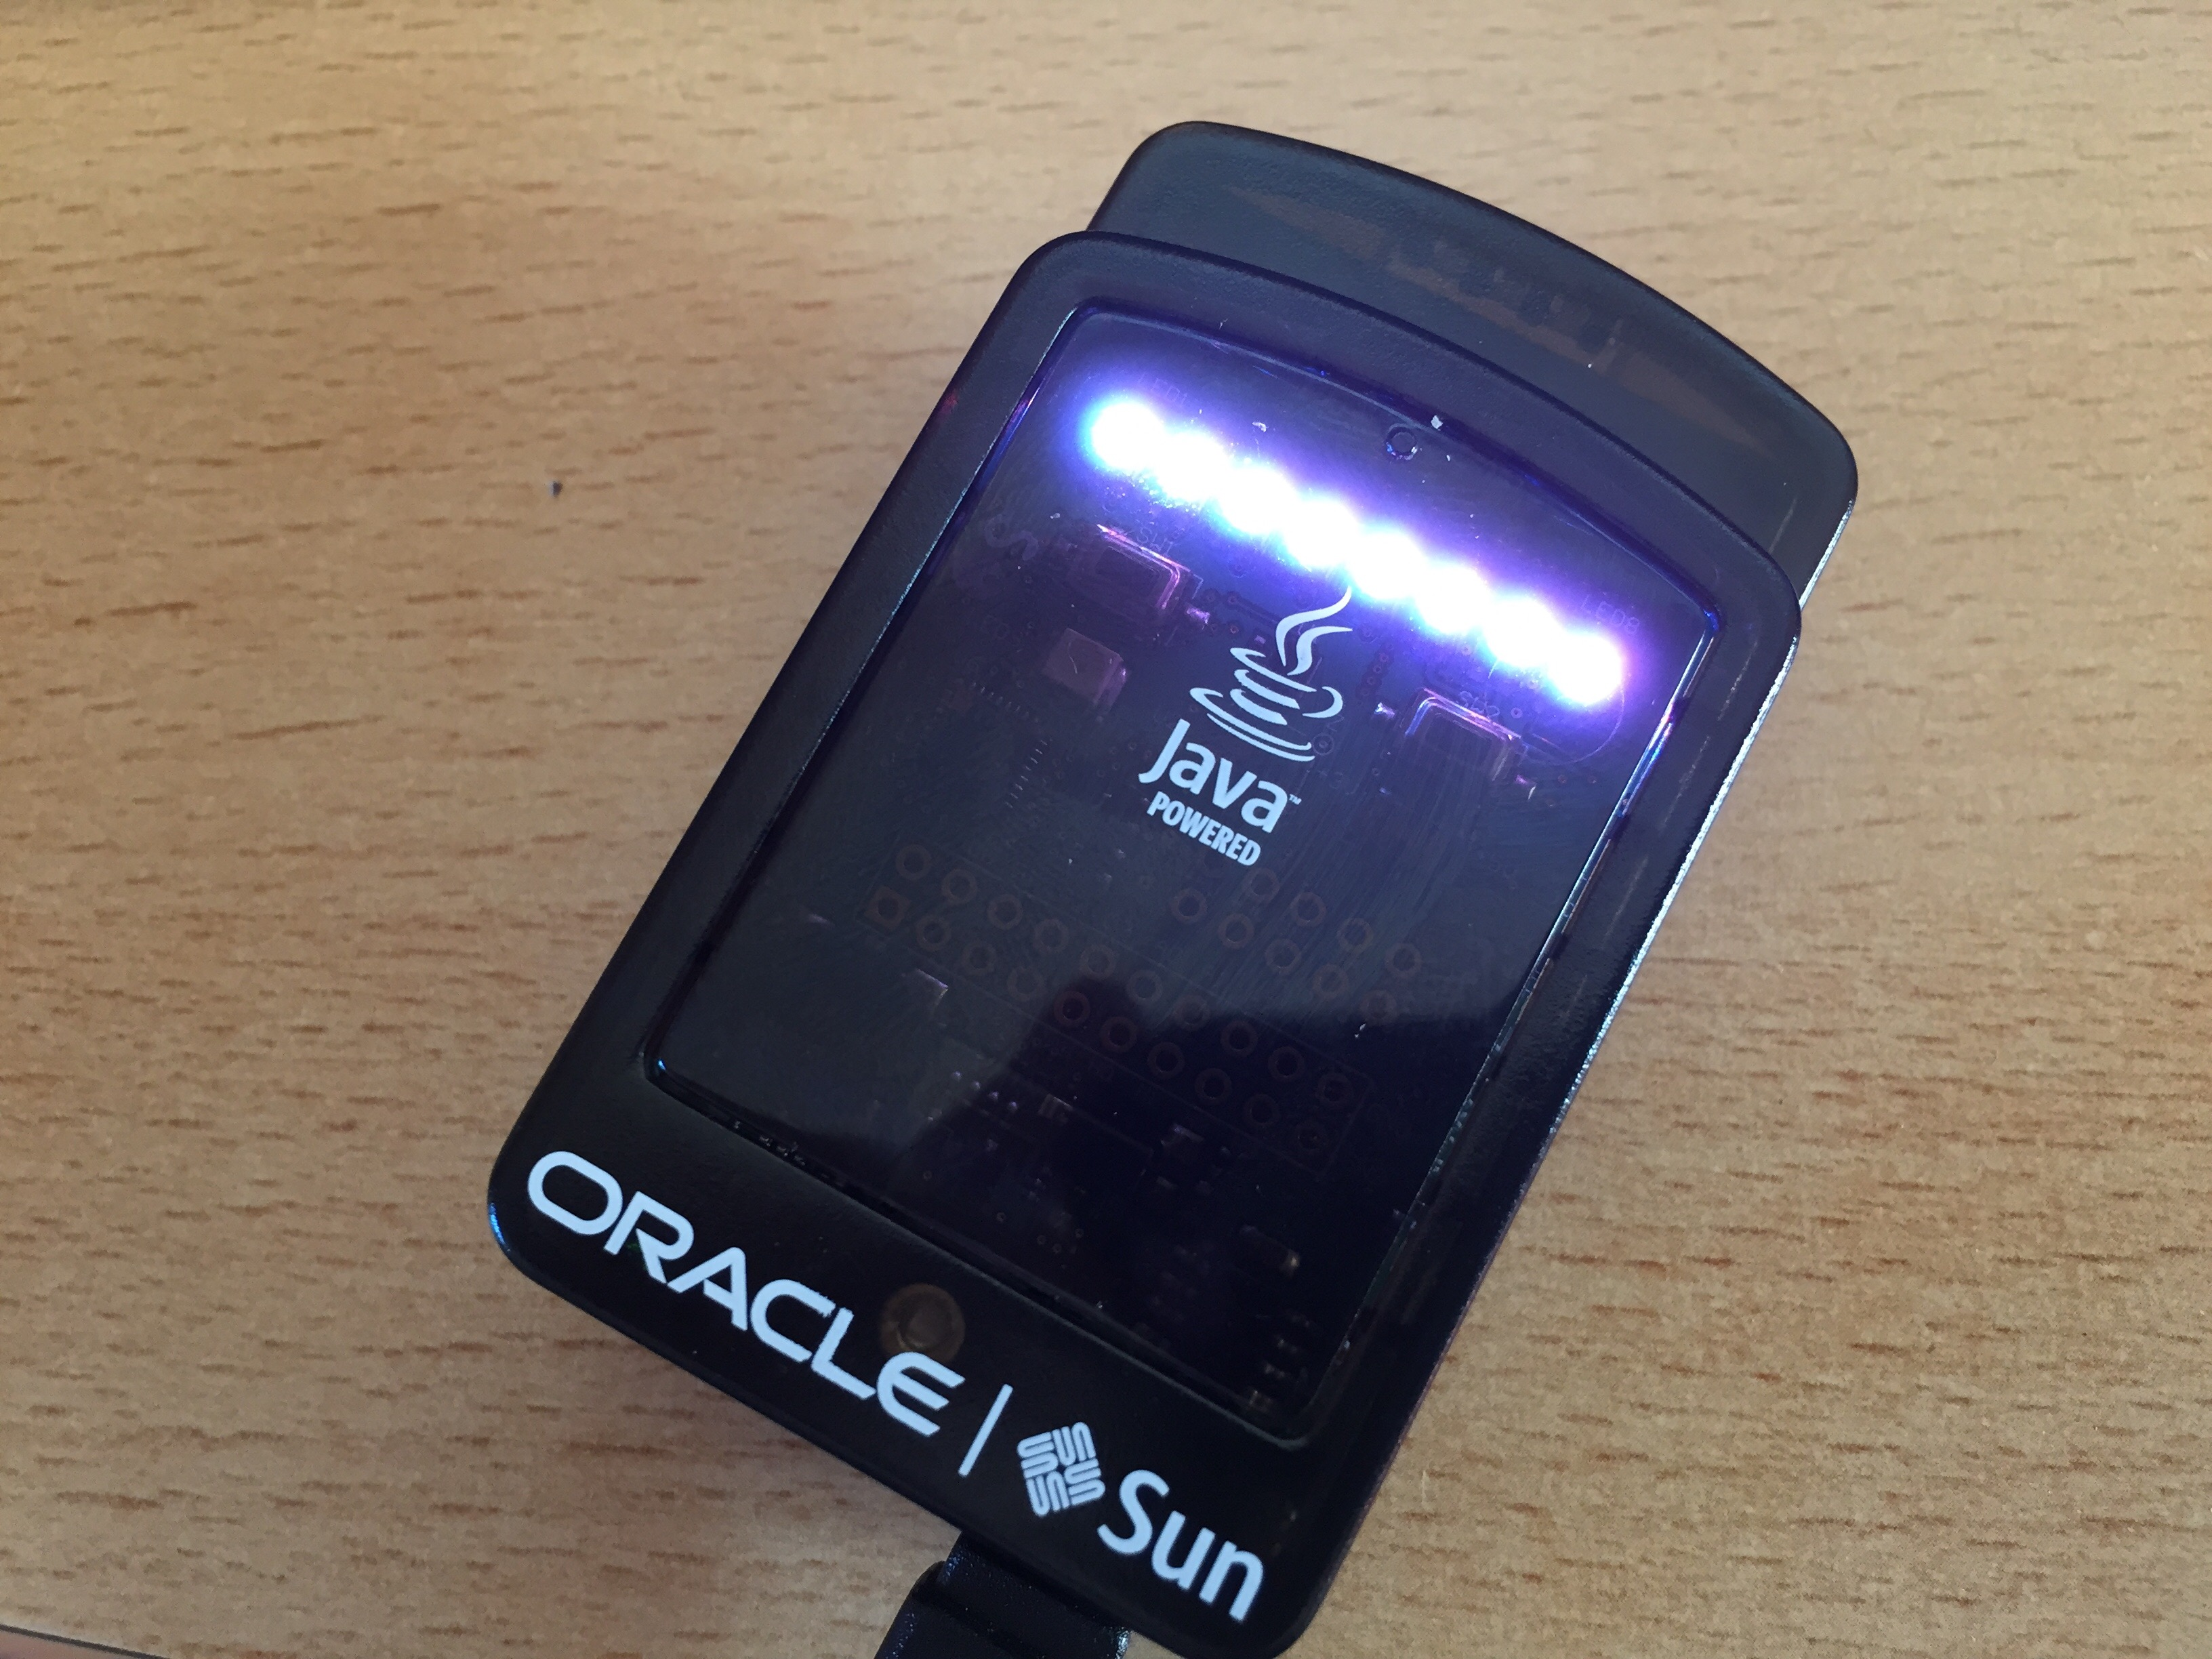
\includegraphics[scale=0.08]{Bilder/uebung1}
	\caption{Leuchtende LEDs des 'Flashlight'-Programms}
	\label{f:uebung1}
\end{figure}

Für die geplante Raumüberwachung ist diese Übung insofern hilfreich, als das hier der Umgang mit den LEDs und deren Verhalten auf äußere Einflüsse gezeigt wurde. In der späteren Implementierungsphase der Raumüberwachung sollen LEDs anzeigen, ob eine Bewegung und somit ein illegales Eindringen in den Raum stattfand.

\section{Implementierung einer Raum\"uberwachung}\label{s:ImplementierungRaumueberwachung}

\subsection{Idee}\label{ss:Idee}

Nicht nur für Museen, Villen oder Betriebe ist ein Sicherheitssystem sinnvoll, denn besonders in private Wohnungen und Häuser wird gerne eingebrochen.

\begin{figure}[H] 
	\centering
	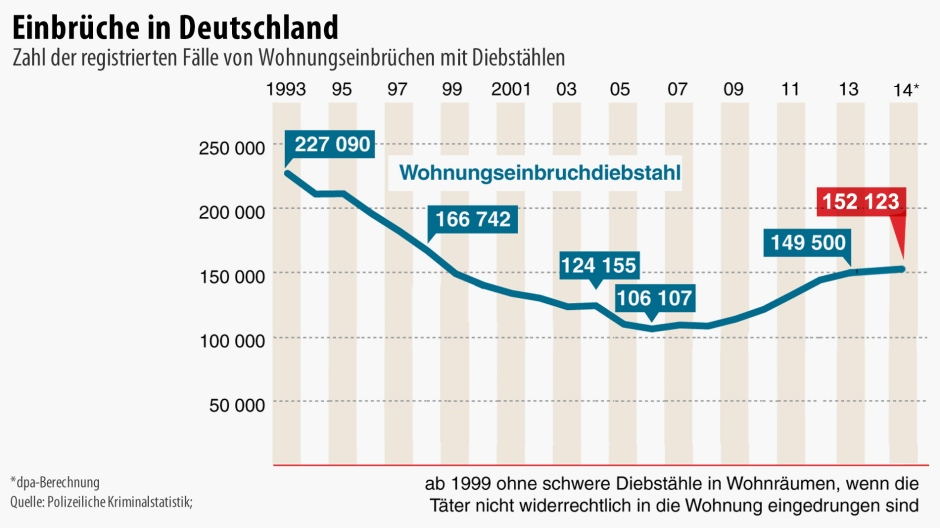
\includegraphics[scale=0.35]{Bilder/einbrueche}
	\caption{Einbruchsstatistik in Deutschland\cite{i:einbrueche}}
	\label{f:einrbrueche}
\end{figure}

Allein im Jahr 2014 wurde über 150.000 mal in Deutschland ein Einbruch mit Diebstahl gemeldet. Die Aufklärungsrate der Verbrechen hingegen ist jedoch sehr gering. Um sich vor solchen Straftaten zu schützen werden Überwachungsanlagen immer beliebter.\\
Im Rahmen dieser Studienarbeit soll eine Raumüberwachung entwickelt werden, die mit Hilfe von untereinander vernetzten Sensoren Einbrüche frühzeitig erkennt, und an den Besitzer meldet. Die Überwachung soll direkt an Fenster und Türen stattfinden, mit Hilfe von Vibrationssensoren, Mikrophonen oder Kameras sollen außergewöhnliche Vorkommnisse ausgewertet werden. Bei einem Einbruch kann dies dem Besitzer über das Netzwerk mitgeteilt werden.


\subsection{Umsetzung}\label{s:Umsetzung}

Im Rahmen der Studienarbeit wurden mit der NetBeans IDE und der Programmiersprache Java zwei Applikationen erstellt, welche einen ersten Ansatz für eine Einbruchsicherung realisieren. Sie sind beliebig erweiterbar, so dass diese als Grundlage für eine komplexere Raumüberwachung dienen können. Die Gesamtimplementation wurde in zwei Teilapplikationen aufgeteilt. Die erste Applikation ist die ‚Desktop-Applikation‘, welche auf dem Rechner läuft und die Daten vom SunSPOT-Sensor empfängt. Auf dem SunSPOT läuft der zweite Teil der Implementation, welcher Bewegungen des Sensors feststellt und diese an eine SunSPOT-Basisstation weiterleitet. In den folgenden Abschnitten wird die genauere Funktionsweise der zwei Teilapplikationen behandelt.

\subsubsection{Desktop-Applikation}\label{sss:Desktop-Applikation}

Die Desktop-Applikation der praktischen Arbeit umfasst knapp 100 Zeilen und dient zum Aufbau einer Radiogram-Verbindung zwischen SunSPOT und Basisstation sowie zum Empfang der vom SPOT gesendeten Daten. 

\begin{lstlisting}[language=Java,caption={Ausschnitt aus der setup()-Methode},label=lst:setup,frame=single] 
private void setup() {
	fr = new JFrame("Einbruchsicherung");
	status = new JTextArea();
	JScrollPane sp = new JScrollPane(status);
	fr.add(sp);
	fr.setSize(360, 200);
	fr.validate();
	fr.setVisible(true);
}           
\end{lstlisting}

Im ersten Schritt wird die Methode ‚setup()‘ definiert, welche zur besseren Visualisierung der Informationen einen JFrame erstellt, in welchen nachher eingetragen werden kann, dass der Sensor eine Bewegung erfahren hat. Sie wird zum Start des Programms aufgerufen, damit das Fenster auch entsprechend erstellt wird. \\

Des weiteren ist eine Methode ‚run()‘ vorhanden, welche direkt nach der ‚setup()‘-Prozedur aufgerufen wird. Diese Funktion kümmert sich sowohl um das Öffnen eines serverseitigen Ports als auch um den Empfang von Datenpaketen, welche an diesen Port versendet werden. \\
Um Daten vom Sensor empfangen zu können, muss in der Desktop-Applikation auf einem selbst festgelegten Port nach Verbindungen ‚gelauscht‘ werden. 
\\
\begin{lstlisting}[language=Java,caption={Öffnen des serverseitigen Ports},label=lst:portserver,frame=single] 
try {
	// Oeffnen einer Radiogram-Verbindung auf der Desktop-Seite
	// um Daten von Sensoren empfangen zu koennen
	rCon = (RadiogramConnection) Connector.open("radiogram://:" + HOST_PORT);
	dg = (Radiogram)
	rCon.newDatagram(rCon.getMaximumLength());
	} 
	
catch (Exception e) {
	System.err.println("setUp caught " + e.getMessage());
	throw e;
}
\end{lstlisting}

Der oben gezeigte Codeausschnitt eröffnet einen serverseitigen Port mit Hilfe der vorher festgelegten HOST\_PORT Variable und lauscht nun fortan auf diesem für Pakete, die vom SunSPOT an die Basisstation versendet werden.\\

\begin{figure}[H] 
	\centering
	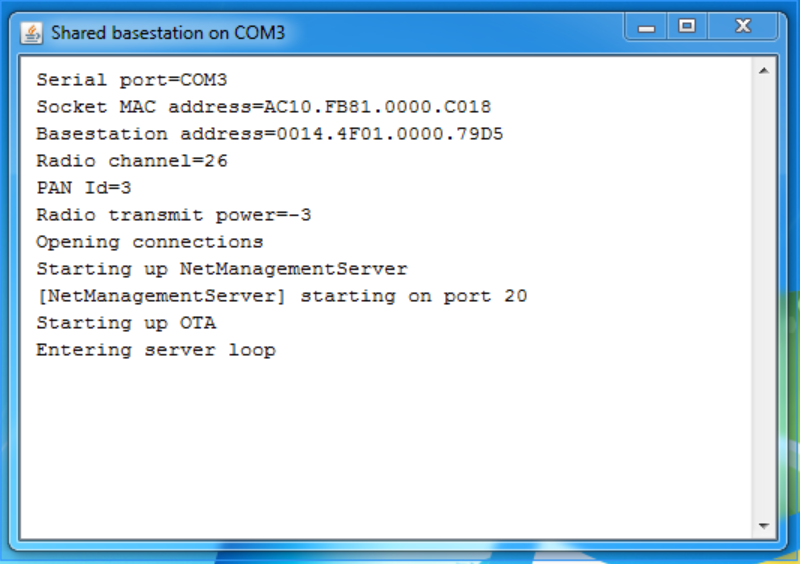
\includegraphics[scale=0.5]{Bilder/server}
	\caption{Logdaten der Basisstation bei Servererstellung}
	\label{f:server}
\end{figure}

Der zweite Teil der ‚run()‘-Methode besteht aus einer while-Schleife, welches auf ankommende Pakete wartet und diese entgegennimmt. Nur wenn der SPOT eine Bewegung erfährt, sendet er ein Paket an die Basisstation. So kann die Desktop-Applikation sicher sein, dass immer, wenn ein Paket gesendet wird, eine Bewegung stattfand.\\

\begin{lstlisting}[language=Java,caption={Auswerten des empfangenen Paketes},label=lst:rcvpackage,frame=single] 
while (true) {
	try {
		// Empfangen und Lesen des Pakets
		rCon.receive(dg);
		long time = dg.readLong();
		System.out.println(time);
		status.append("Bewegung festgestellt!\n");
		} 
	catch (Exception e) {
		System.err.println("Exception " + e +  " beim Lesen der Daten.");
		throw e;
		}
	}
\end{lstlisting}

Innerhalb des übermittelten Paketes befindet sich die aktuelle Uhrzeit, um die Bewegung nachher genau zeitlich einordnen zu können. Sobald die Desktop-Applikation ein Paket empfängt, gibt sie auf dem Bildschirm innerhalb des erstellten Frames den Text 'Bewegung festgestellt!' aus. So wird dem Nutzer unmissverständlich klar gemacht, dass der Sensor in Bewegung war.

\begin{figure}[H] 
	\centering
	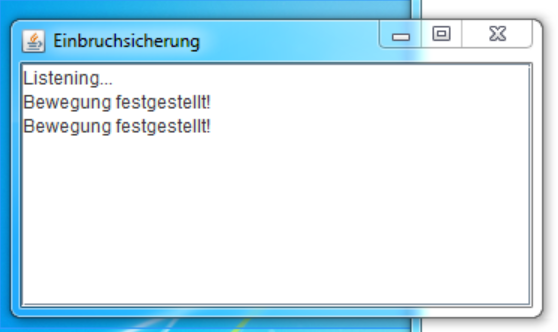
\includegraphics[scale=0.8]{Bilder/bewegung}
	\caption{JFrame mit textueller Ausgabe}
	\label{f:bewegung}
\end{figure}

Innerhalb der Konsole werden neben Debugausgaben zur Basisstation und die Liste eröffneter Ports der Zeitstempel, welcher mit der Bewegung vom SunSPOT übermittelt wird, ausgegeben.

\begin{figure}[H] 
	\centering
	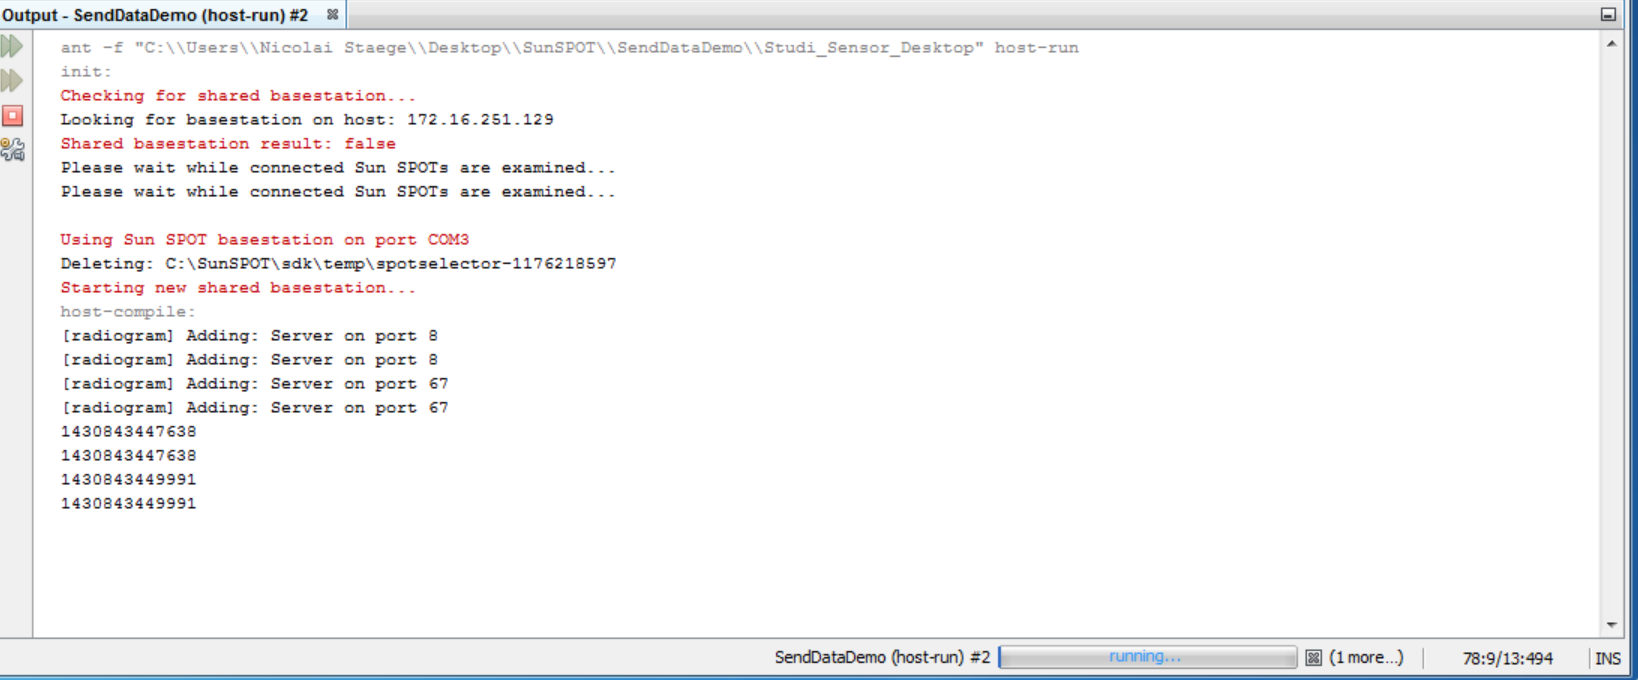
\includegraphics[scale=0.5]{Bilder/timestamp}
	\caption{Konsolenausgabe mit Timestamp}
	\label{f:timestamp}
\end{figure}

\subsubsection{SPOT-Applikation}\label{sss:SPOT-Applikation}

\section{Erweiterungsm\"oglichkeiten}\label{s:Erweiterungsmoeglichkeiten}

Das entwickelte System kann durch mehrere Komponenten erweitert werden. Hierbei handelt es sich um drei Hauptkategorien: Die Visualisierung, weitere Sensoren und eine Benachrichtigung des Wohnungsbesitzers.

\subsection{Visualisierung mithilfe eines Webservers}\label{ss:visualisierung}



Durch die Kombination der SunSpot-Sensoren mit einem kleinen Computer lässt sich das System mit einer interaktiven Visualisierung erweitern. Hierbei erhält der Computer von der SunSpot-Basisstation Informationen über die Umgebung. Dies können beispielsweise die aufgezeichneten Vibrationen der Sensoren sein.\\
Auf dem Computer wird ein Webserver eingerichtet, der mit den erhaltenen Informationen eine Webseite erstellt, auf die der Besitzer zugreifen kann. Hier erhält er einen Überblick über den Status seiner Wohnung und besitzt die Möglichkeit mit dem Sicherheitssystem zu interagieren. 

\begin{figure}[H] 
	\centering
	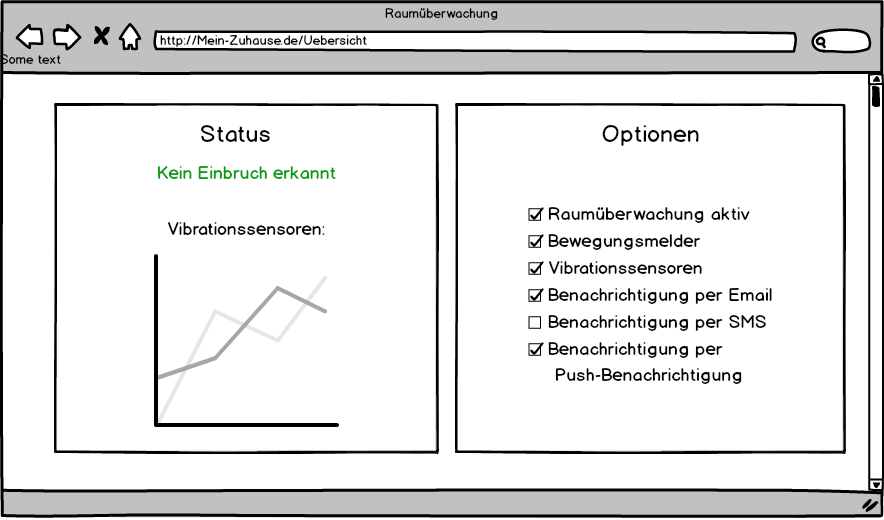
\includegraphics[scale=0.4]{Bilder/mockupwebsite}
	\caption{Mockup einer Webseite}
	\label{f:mockupwebsite}
\end{figure}
\todo[inline]{"Created with" herausnehmen}

Die Umsetzung dieser Erweiterung ist mithilfe eines Raspberry Pis möglich. Dieser besitzt einen USB-Anschluss, über den die Basisstation der SunSpots angeschlossen werden kann. Zusätzlich kann sich der Raspberry Pi über Ethernet oder WLAN mit dem Internet verbinden.\\
Mithilfe der Debian-Linux Distribution Raspbian kann ein Tomcat- oder Apache Webserver aufgesetzt werden, der die Webseite des Überwachungssystems bereitstellt. Auf der Webseite kann dem Besitzer das Aktivieren, sowie Deaktivieren der Überwachung oder einzelner Sensoren ermöglicht werden.

\begin{figure}[H] 
	\centering
	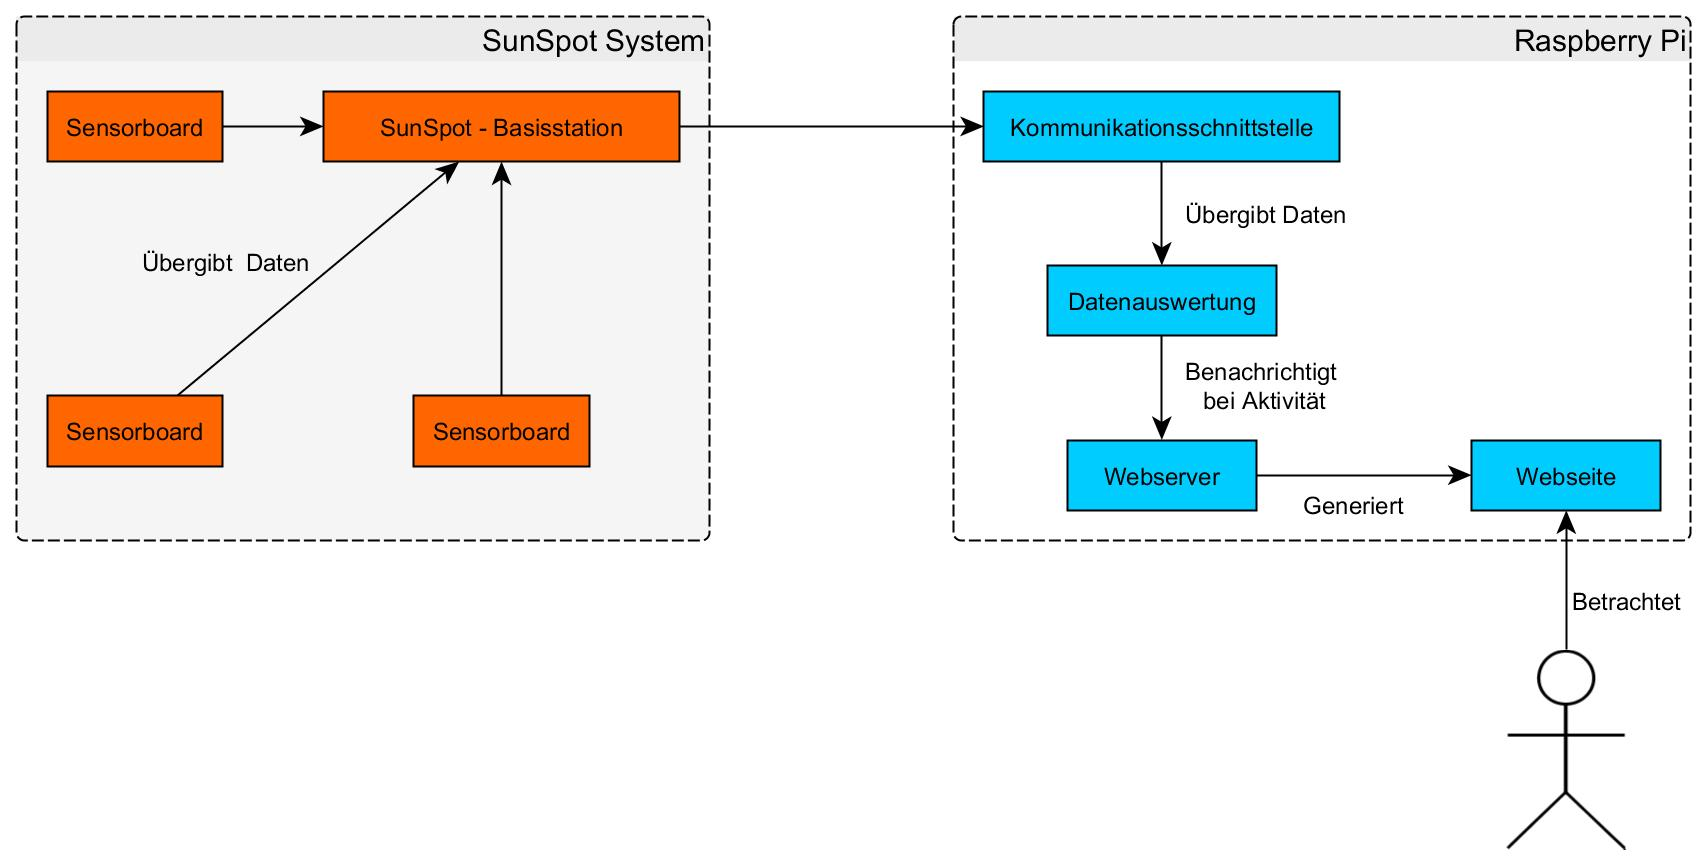
\includegraphics[scale=0.25]{Bilder/Visualisierung}
	\caption{Visualisierung mithilfe eines Raspberrys und Webserver}
	\label{f:visualisierung}
\end{figure}
\subsection{Erweiterung durch verschiedene Sensoren}\label{ss:sensoren}

Eine Erweiterungsmöglichkeit ist die Ergänzung verschiedener Sensoren. 
Durch ein Mikrophon können ungewöhnliche Geräusche aufgezeichnet werden. Diese können von Einbruchsversuchen an einer Tür oder durch eine zerbrechende Scheibe entstehen. Eine großer Vorteil eines Mikrophons ist, das auch jegliche Kommunikation der Einbrecher aufgezeichnet werden kann. So kann ebenfalls entschieden werden, ob es sich um einen Einbrecher handelt, oder ob Verwandtschaft mit einem Ersatzschlüssel die Wohnung betreten hat.\\

Durch Bewegungsmelder werden häufig Beleuchtungen, in diesem Szenario kann er jedoch zur Einbruchserkennung verwendet werden: Falls sich etwas bewegt, jedoch niemand zu hause sein sollte, wird ein Alarm ausgelöst. 
Da die Überwachung durch Ultraschall oder Infrarot geschieht, kann es im Raum auch dunkel sein.\\

Eine weitere Möglichkeit ist das Ergänzen einer Kamera. Diese kann entweder als Bewegungsmelder eingesetzt werden, oder Bilder und Videos der Wohnung aufnehmen. Im Falle eines Einbruchs kann so der Täter direkt photographiert werden. Dies  Ermöglicht eine gezielte strafrechtliche Verfolgung. Die Kamera kann jedoch auch auf Wunsch des Wohnungsbesitzers Bild- oder Videomaterial aufzeichnen, dass über das Internet einsehbar ist. Auf diese Weise kann man einen Blick in die Wohnung werfen, ohne anwesend zu sein.

Die verschiedenen Sensoren können beispielsweise an einen Raspberry Pi angeschlossen werden, der die Eingangssignale überwacht, und bei ungewöhnlichen Werten anschlägt.

\begin{figure}[H] 
	\centering
	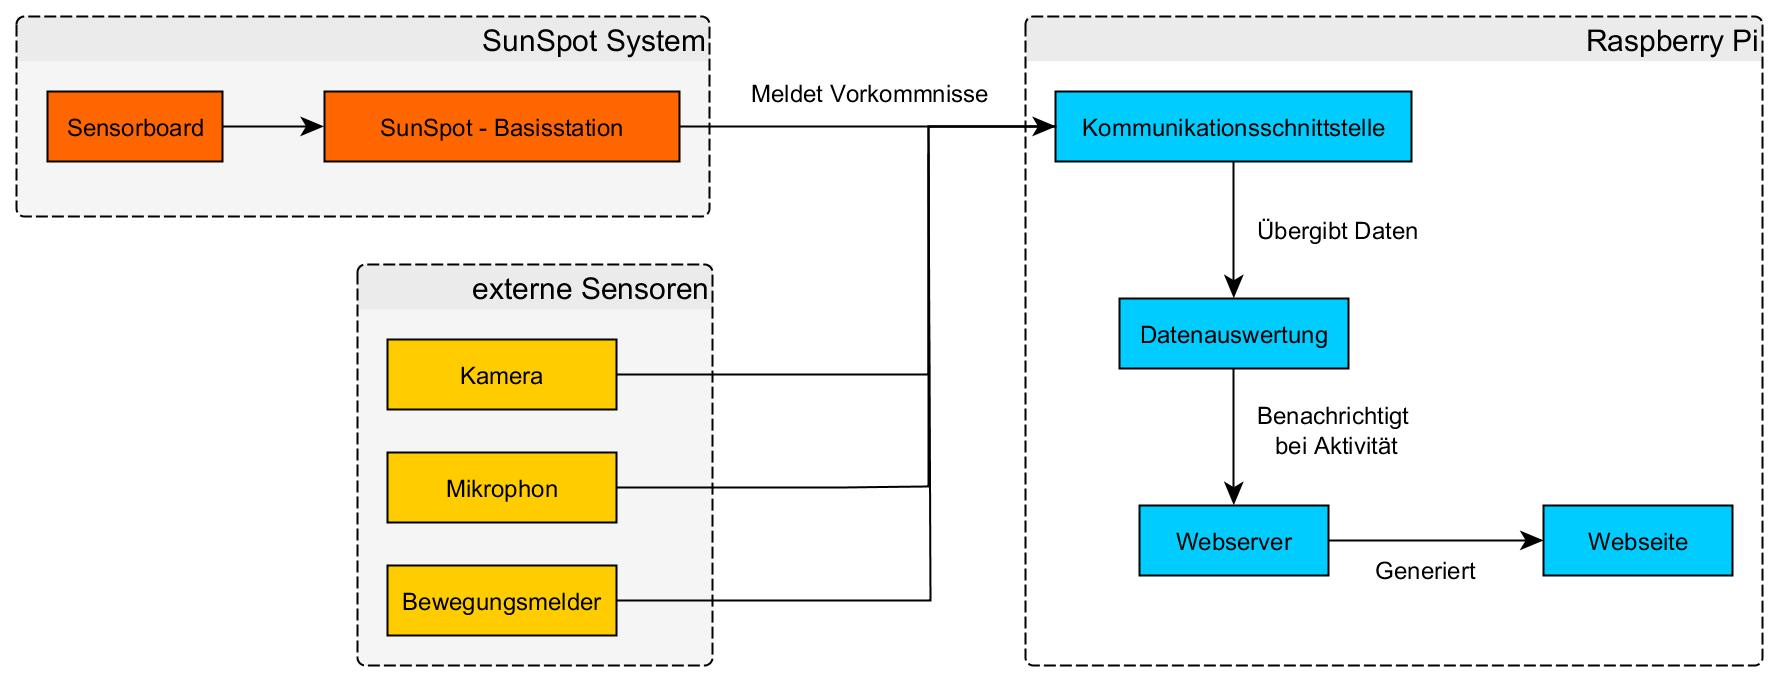
\includegraphics[scale=0.22]{Bilder/extSensor}
	\caption{Aufbau eines Sensornetzes mithilfe eines Raspberry Pis}
	\label{f:extSensor}
\end{figure}
\subsection{Benachrichtigung des Benutzers}\label{ss:benachrichtigung}